\scanpage{59}
\figure{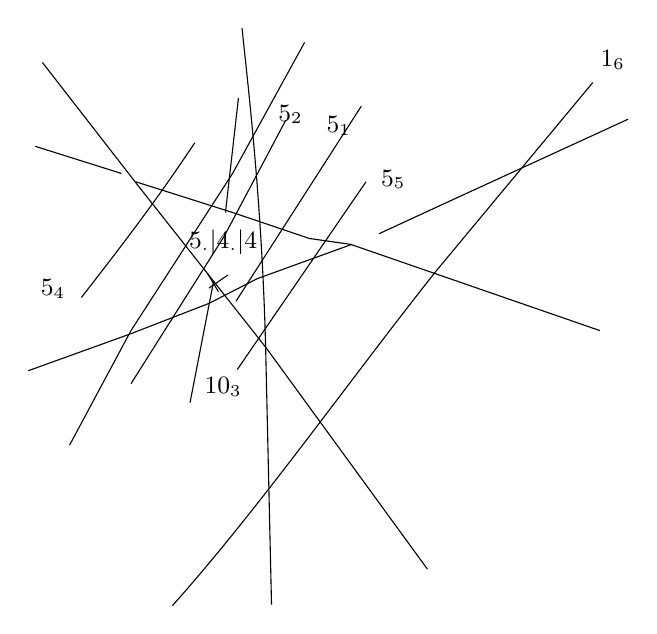
\begin{tikzpicture}[x=.015cm,y=-.015cm,every node/.style={font=\small,inner sep=0pt}]
\draw (148,67) -- (228,170) -- (337,308) -- (474,496);
\draw (142,138) -- (215,161); \draw (227,168) -- (309,194) -- (374,216) -- (409,221) -- (620,294);
\draw (136,328) -- (222,297) -- (289,271) -- (330,250) -- (410,221); \draw (433,212) -- (498,182) -- (644,115);
\draw (181,266) .. controls (216,221) and (243,186) .. (277,135);
\draw (171,391) -- (223,294) -- (309,161) -- (370,50);
\draw (223,339) -- (302,214) -- (354,116);
\draw (273,355) -- (293,252); \draw (303,194) -- (314,97);
\draw (312,269) -- (418,104); \draw (313,327) -- (422,168);
\draw (317,38) .. controls (324,103) and (334,193) .. (337,308) -- (342,526);
\draw (258,527) .. controls (332,444) and (405,340) .. (481,244) -- (614,84);
\node at (157,259) {$5_4$}; \node at (358,111) {$5_2$};
\node at (399,121) {$5_1$}; \node at (445,166) {$5_5$};
\node at (301,219) {$\unsure{5_{.}|4_{.}|4}$};
\draw (288,246) -- (297,261); \draw (289,258) -- (305,247);
\node at (301,342) {$10_3$}; \node at (631,65) {$1_6$};
\end{tikzpicture}}
\[
\begin{array}{rl}
5 &\\
15 &=5+10\\
10 &=5+5\\
1 &\\ \cline{1-1}
31 &
\end{array}
\]
\[
\begin{aligned}
1_6&\equiv\text{icosaèdre}\\
5_1&\equiv\text{hexagone}\\
5_4,5_2&\equiv\text{triangle bordé}\\
5_5,10_3&\equiv\text{carré gammé}
\end{aligned}
\]
% archive sheet number: 58
